\subsection{Pagineren}

Pagineren is het geheugen opdelen in kleine stukken van vaste grootte en welke allemaal even groot zijn. Deel nu elk proces op in stukken van dezelfde grootte. Dergelijke stukken worden pagina’s genoemd. De stukken van het geheugen worden frames genoemd.

Het besturingssysteem houdt een pagina tabel bij voor elk proces. Deze tabel bevat

\begin{itemize}
\item De frame locatie voor elke pagina in het proces
\item Een geheugenadres bestaande uit een paginanummer en een offset binnen die pagina.
\end{itemize}


\begin{figure}[htp]
    \centering
            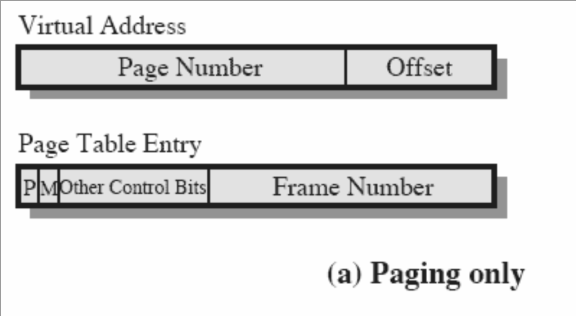
\includegraphics[width=4in]{img/pagineren.png}
        \caption{Paging only}
    \label{fig:Paging only}
\end{figure}


\begin{figure}[htp]
    \centering
            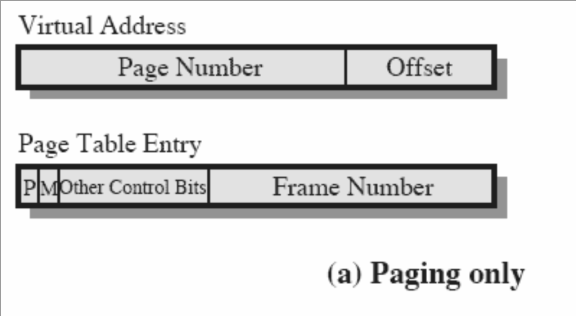
\includegraphics[width=4in]{img/pagineren.png}
        \caption{Paging only}
    \label{fig:Paging only}
\end{figure}

Bovenstaande figuur illustreert het gebruik van pagina’s en frames. Op een bepaald moment zijn sommige frames in het geheugen bezet en zijn andere vrij. Het besturingssysteem houdt een lijst bij van vrije frames. De figuur verduidelijkt zichzelf.

Voor adresvertaling bij paginering zijn volgende stappen nodig:

\begin{itemize}
\item Haal het paginanummer uit de linker in bits van het logische adres
\item Gebruik het paginanummer als inde in de procespaginatabel om het framenummer k te vinden.
\item Het fysieke beginadres van het frame is k * 2m, en het fysieke adres van de gezochte byte is gelijk aan dit nummer plus de positie. Dit fysieke adres hoeft niet te worden berekend. Het wordt eenvoudig gevormd door het framenummer toe te voegen aan de positie.
\end{itemize}

